\chapter{Implementation of the Custom Abstraction Software and Experimental Results} \label{ch:implement}

The abstraction procedure can be fully scripted using the computer algebra tool 
{\sc Singular}. However, {\sc Singular} has limitations which make abstraction
of large circuits {\it impossible}. This is due to:
\begin{itemize}
\item A limit on the number of ring variables allowed. As of {\sc Singular} release 4.0.1, 
a ring cannot be declared with more than $32,767$ variables. This limits the number
of gates that can be present in the design.
\item The size of an exponent $(n)$ of a variable $x$, is limited $n<2^{32}$.
\item Large amount of memory usage and slow computation time. 
{\sc Singular} uses a dense-distributive structure for polynomials, which is a poor 
representation of sparse polynomials over rings with many variables.
\end{itemize}
The limit on the size of exponents prohibits an abstraction beyond $32$-bit circuits,
as larger circuits require manipulating word-level variables with exponents 
larger than $2^{32}$. Even
if this limitation is overcome, Singular uses an enormous amount of memory.
For instance, preliminary experiments show that using Singular to compute the
initial reduction of a $163$-bit Mastrovito multiplier uses $41.6$ GB of memory!
Thus, deriving abstractions using Singular is infeasible on 
desktop workstations.

In order to overcome these limitations, a custom C++ tool is developed to 
compute the word-level abstraction of circuits quickly and efficiently. 
This chapter describes the implementation details of this tool.

\section{Data Structures and Algorithms}

Computing a word-level abstraction requires the representation and manipulation 
of polynomials in $\Fkk[x_1,\dots,x_d]$ over a lex ordered ring. 
Intermediate polynomials can become 
very large during the abstraction procedure, so the data structure to represent them 
is designed to 
conserve memory while allowing for fast manipulation during the reduction 
procedures. The backbone of the tool is a custom library composed of three main
sections:
\begin{enumerate}
\item Galois field elements
\item Monomials and rings
\item Polynomials and division procedures
\end{enumerate}
These are built on top of each other. The starting point is the custom 
Galois field element section, which facilitates the construction of 
Galois field elements over $\Fkk$.

\subsection{Galois Field Elements}

The Galois field section of the library is initialized by parsing a given primitive polynomial $P(x)$
of degree $k$ which constructs $\Fkk$. Any element $C \in \Fkk$ can be represented 
in the form 
\begin{equation}
C = c_{k-1}\cdot\alpha^{k-1}+c_{k-2}\cdot\alpha^{k-2}+\cdots+c_2\cdot\alpha^2+c_1\cdot\alpha+c_0
\end{equation}
where 
$\{c_0,\dots,c_{k-1}\}\in\F_2$ and $\alpha$ is the primitive element. This {\it structure}
is stored as an unsigned byte array containing $\{c_0,\dots,c_{k-1}\}$, 
as shown in Figure \ref{fig:gfStruct}. Thus, each element uses $\left\lfloor\frac{k-1}{8}\right\rfloor+1$ 
bytes of memory. 
Any leading bits after $c_{k-1}$ in the last byte are set to $0$.
\begin{figure}[h]
	\begin{center}
	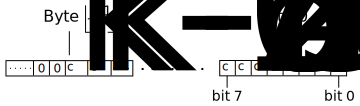
\includegraphics[scale=1]{figures/gfElementStructure}
	\end{center}
	\caption{Object structure of a Galois field element}
	\label{fig:gfStruct}
\end{figure}

{\it Addition} between two elements
\begin{eqnarray}
C&=&c_{k-1}\cdot\alpha^{k-1}+\cdots+c_2\cdot\alpha^2+c_1\cdot\alpha+c_0 \\
D&=&d_{k-1}\cdot\alpha^{k-1}+\cdots+d_2\cdot\alpha^2+d_1\cdot\alpha+d_0
\end{eqnarray}
is simply a combination of like terms
\begin{equation}
C+D=(c_{k-1}+d_{k-1})\cdot\alpha^{k-1}+\cdots+(c_2+d_2)\cdot\alpha^2+(c_1+d_1)\cdot\alpha+(c_0+d_0)
\end{equation}
Since addition over $\F_2$ is computed as a bit-wise XOR, the library's Galois field element 
structure allows addition to be trivially performed as a byte-wise XOR operation. 
Furthermore, this structure makes it easy to check if a given element is equal 
to $0$ or $1$, which is used in deciding when a term is to be removed ($0$) and when 
a division can be ignored ($1$).

During {\it library initialization}, the elements 
$\alpha^k,\alpha^{k+1},\dots,\alpha^{2k-2}$ are pre-computed and cached. First,
$\alpha^k$ is derived directly from the given primitive polynomial, 
\begin{equation}
P(x)=x^k+c_{k-1}\cdot x^{k-1}+\cdots+c_1\cdot x+1
\end{equation}
for $\{c_1,\dots,c_{k-1}\}\in\F_2$. Since $P(\alpha)=0$,
\begin{equation}
\alpha^k=c_{k-1}\cdot\alpha^{k-1}+\cdots+c_1\cdot\alpha+1
\end{equation}
To compute $\alpha^{k+1}$, first compute a $1$-bit left shift of
$\alpha^k$.
\begin{equation}
\alpha^{k+1}=c_{k-1}\cdot\alpha^k+c_{k-2}\cdot\alpha^{k-1}+\cdots+c_1\cdot\alpha^2+\alpha
\end{equation}
This element can contain the term $\alpha^k$, which must be minimized by the primitive
polynomial.
Thus, if $c_{k-1}$ is $1$, the $c_{k-1}\alpha^k$ term is removed and the minimized 
form of $\alpha^k$ is added. This derives the minimized form for $\alpha^{k+1}$. 
Computation continues in this fashion (shift by 1, minimize if needed) until all
$\alpha^k,\alpha^{k+1},\dots,\alpha^{2k-2}$ have been derived.
These elements are later used during the multiplication procedure.

\begin{Example}
\label{ex:gf4init}
Given the primitive polynomial $P(x)=x^4+x^3+1$, initialize the library by computing
$\alpha^4,\alpha^5,$ and $\alpha^6$. Here, $k=4$, and each element of $\F_{2^4}$ can be 
represented as
\begin{equation}
c_3\cdot\alpha^3+c_2\cdot\alpha^2+c_1\cdot\alpha+c_0
\end{equation}
which is stored as one byte in the following form.
\begin{equation}
\begin{tabular}{|c|c|c|c|c|c|c|c|} 
\hline
$0$ & $0$ & $0$ & $0$ & $\mathbf{c_3}$ & $\mathbf{c_2}$ & $\mathbf{c_1}$ & $\mathbf{c_0}$ \\
\hline
\end{tabular}
\end{equation}
Notice that there are $4$ leading bits which are unused; these are always set to $0$.

$P(\alpha)=\alpha^4+\alpha^3+1=0$. Hence, $\alpha^4=\alpha^3+1$, 
which is stored as
\begin{equation}
\begin{tabular}{cc|c|c|c|c|c|c|c|c|} 
\multicolumn{6}{c}{}&\multicolumn{1}{c}{$c_3$}&\multicolumn{1}{c}{$c_2$}&\multicolumn{1}{c}{$c_1$}&\multicolumn{1}{c}{$c_0$} \\
\hhline{~~--------}
$\alpha^4$&$=$&$0$ & $0$ & $0$ & $0$ & $\mathbf{1}$ & $\mathbf{0}$ & $\mathbf{0}$ & $\mathbf{1}$ \\
\hhline{~~--------}
\end{tabular}
\end{equation}
To compute $\alpha^5$, take the $\alpha^4$ element and
shift the result left 1 bit. The $c_3$ term is dropped since the leading $4$ 
bits are always $0$.
\begin{equation}
\begin{tabular}{|c|c|c|c|c|c|c|c|} 
\hline
$0$ & $0$ & $0$ & $0$ & $\mathbf{0}$ & $\mathbf{0}$ & $\mathbf{1}$ & $\mathbf{0}$ \\
\hline
\end{tabular}
\end{equation}

Then, since $c_3$ was $1$, add $\alpha^4$.
\begin{equation}
\begin{tabular}{c|c|c|c|c|c|c|c|c|} 
\hhline{~--------}
&$0$ & $0$ & $0$ & $0$ & $\mathbf{0}$ & $\mathbf{0}$ & $\mathbf{1}$ & $\mathbf{0}$ \\
\hhline{~========}
$+$&$0$ & $0$ & $0$ & $0$ & $\mathbf{1}$ & $\mathbf{0}$ & $\mathbf{0}$ & $\mathbf{1}$ \\
\hhline{~--------}\multicolumn{9}{c}{}\\
\hhline{---------}\multicolumn{9}{c}{}\\
\hhline{~--------}
&$0$ & $0$ & $0$ & $0$ & $\mathbf{1}$ & $\mathbf{0}$ & $\mathbf{1}$ & $\mathbf{1}$ \\
\hhline{~--------}
\end{tabular}
\end{equation}
This gives $\alpha^5=\alpha^3+\alpha+1$. Similarly, $\alpha^6$ is derived as
\begin{equation}
\begin{tabular}{c|c|c|c|c|c|c|c|c|} 
\hhline{~--------}
&$0$ & $0$ & $0$ & $0$ & $\mathbf{0}$ & $\mathbf{1}$ & $\mathbf{1}$ & $\mathbf{0}$ \\
\hhline{~========}
$+$&$0$ & $0$ & $0$ & $0$ & $\mathbf{1}$ & $\mathbf{0}$ & $\mathbf{0}$ & $\mathbf{1}$ \\
\hhline{~--------}\multicolumn{9}{c}{}\\
\hhline{---------}\multicolumn{9}{c}{}\\
\hhline{~--------}
&$0$ & $0$ & $0$ & $0$ & $\mathbf{1}$ & $\mathbf{1}$ & $\mathbf{1}$ & $\mathbf{1}$ \\
\hhline{~--------}
\end{tabular}
\end{equation}
\end{Example}

{\it Multiplication} requires temporarily increasing the size of the byte-array to 
store the intermediate result, which can have values up to $\alpha^{2(k-1)}$.
\begin{equation}
c_{2k-2}\cdot\alpha^{2k-2}+\cdots+c_k\cdot\alpha^k+c_{k-1}\cdot\alpha^{k-1}+\cdots+c_2\cdot\alpha^2+c_1\cdot\alpha+c_0
\end{equation}
This result needs to be divided by the given minimum polynomial. Each $\alpha$ 
term with an exponent of $k$ or larger is replaced by its minimized equivalent,
which was computed during initialization. That is, for $i\geq k$, each term for which $c_{i}=1$ 
is removed and the minimized form of $\alpha^i$ added in.

\begin{Example}
\label{ex:gf4mult}
Consider again the setup for $\F_{2^4}$ from Example \ref{ex:gf4init}. Compute the
product of the following two elements:
\begin{eqnarray}
\alpha^3+\alpha^2+1 \\
\alpha^2+\alpha
\end{eqnarray}
These elements are stored respectively as
\begin{eqnarray}
\begin{tabular}{|c|c|c|c|c|c|c|c|} 
\hline
$0$ & $0$ & $0$ & $0$ & $\mathbf{1}$ & $\mathbf{1}$ & $\mathbf{0}$ & $\mathbf{1}$ \\
\hline
\end{tabular} \\
\begin{tabular}{|c|c|c|c|c|c|c|c|} 
\hline
$0$ & $0$ & $0$ & $0$ & $\mathbf{0}$ & $\mathbf{1}$ & $\mathbf{1}$ & $\mathbf{0}$ \\
\hline
\end{tabular}
\end{eqnarray}
The intermediate result is computed using the basic shift-and-add procedure.
\begin{equation}
\begin{tabular}{|c|c|c|c|c|c|c|c|}
\hhline{~~~~----}
\multicolumn{3}{c}{} & & $1$ & $1$ & $0$ & $1$ \\
\hhline{~~~~----}
\multicolumn{3}{c}{} & x & $0$ & $1$ & $1$ & $0$ \\
\hhline{~~~~----}\multicolumn{8}{c}{}\\
\hhline{--------}\multicolumn{8}{c}{}\\
\hhline{~~~~----}
\multicolumn{3}{c}{} & & $0$ & $0$ & $0$ & $0$ \\
\hhline{~~~-----}
\multicolumn{2}{c}{} & & $1$ & $1$ & $0$ & $1$ & \multicolumn{1}{c}{} \\
\hhline{~~-----~}
\multicolumn{1}{c}{} & & $1$ & $1$ & $0$ & $1$ & \multicolumn{2}{c}{} \\
\hhline{~-----~~}
\multicolumn{1}{c|}{$+$} & $0$ & $0$ & $0$ & $0$ & \multicolumn{3}{c}{} \\
\hhline{~----~~~}\multicolumn{8}{c}{}\\
\hhline{--------}\multicolumn{8}{c}{}\\
\hhline{--------}
$0$& $\mathbf{0}$ & $\mathbf{1}$ & $\mathbf{0}$ & $\mathbf{1}$ & $\mathbf{1}$ & $\mathbf{1}$ & $\mathbf{0}$ \\
\hline
\end{tabular}
\end{equation}
The intermediate result of the multiplication is $\alpha^5+\alpha^3+\alpha^2+\alpha$, 
which needs to be further minimized. The value of $\alpha^5$ was determined during
initialization to be $\alpha^3+\alpha+1$. The $\alpha^5$ term from the intermediate
result is removed and the minimized form is added.

\begin{equation}
\begin{tabular}{cc|c|c|c|c|c|c|c|c|} 
\hhline{~~--------}
&&$0$ & $0$ & $0$ & $0$ & $\mathbf{1}$ & $\mathbf{1}$ & $\mathbf{1}$ & $\mathbf{0}$ \\
\hhline{~~========}
&$+$&$0$ & $0$ & $0$ & $0$ & $\mathbf{1}$ & $\mathbf{0}$ & $\mathbf{1}$ & $\mathbf{1}$ \\
\hhline{~~--------}\\
\hhline{----------}\\
\hhline{~~--------}
&&$0$ & $0$ & $0$ & $0$ & $\mathbf{0}$ & $\mathbf{1}$ & $\mathbf{0}$ & $\mathbf{1}$ \\
\hhline{~~--------}
\end{tabular}
\end{equation}

So the minimized result of the product is $\alpha^2+1$.

\end{Example}

{\it Division} of two Galois field elements, $C=\frac{B}{A}$, requires finding 
the multiplicative inverse of the divisor: $C=B\cdot A^{-1}$. To find the inverse, 
the library implements the extended Euclidean algorithm over $\Fkk$, depicted in
Algorithm \ref{alg:eucInv}. The algorithm requires a non-minimized 
representation of the element $P(\alpha)$, so the size of object is temporarily 
increased to allow the storage of the $\alpha^k$ bit.
The function $DIV$ returns the quotient and 
remainder of a Euclidean division; that is, $DIV(A,B)$ returns 
$\{Q,R\}$, where $A=B\cdot Q + R$. This procedure is described in Algorithm \ref{alg:eucDiv};
here, $DEG$ returns the highest degree of a given element in $\Fkk$, 
i.e. $DEG(\alpha^4+\alpha^3+1)$ would return $4$.

\begin{algorithm}[hbt]
\SetAlgoNoLine

 \KwIn{$M:=P(\alpha)$ where $P(x)$ was used to generate $\Fkk$, $A\in\Fkk$}
 \KwOut{$A^{-1}$ over $\Fkk$}
  %%%%%%%%%%%%%%%%%%%%
        $\{Q_0,Q_1\}$ := $\{0,0\}$\;
        $\{R_0,R_1\}$ := $\{M,A\}$\;
        $\{U_0,U_1\}$ := $\{0,1\}$\;
        $i$ := $1$\;
        \While { $R_i \neq 1$ }
        {
                \If { $R_i == 0$ }{{\bf ERROR}: No inverse exists}
                $\{Q_{i+1},R_{i+1}\} := DIV(R_{i-1},R_i)$\;
                $U_{i+1}$ := $(Q_{i+1} \cdot U_i) + U_{i-1}$\;
                $i$ := $i+1$\;
        }
        \Return $U_i$\;
\caption{Inverse of an element over $\Fkk$}\label{alg:eucInv}
\end{algorithm}

\begin{algorithm}[hbt]
\SetAlgoNoLine

 \KwIn{$A,B \in \Fkk$}
 \KwOut{$\{Q,R\}$ such that $A = B\cdot Q + R$}
        $\{Q, R\} := \{0,A\}$\;
        %$d := DEG(B)$\;
        \While { $DEG(R) \geq DEG(B)$ }
        {
                $S$ := $\alpha^{DEG(R)-DEG(B)}$\;
                $Q$ := $Q + S$\;
                $R$ := $R + S\cdot B$\;
        }
        \Return $\{Q,R\}$\;
\caption{$DIV$ (Euclidean Division over $\Fkk$)}\label{alg:eucDiv}
\end{algorithm}

\begin{Example}
Given $P(x)=x^8+x^4+x^3+x+1$ which generates $\F_{2^8}$, find $A^{-1}$ where
$A=\alpha^6+\alpha^4+\alpha+1$. Table \ref{tab:divExTab} shows the steps 
Algorithm \ref{alg:eucDiv} goes through to find the inverse.

\begin{table}[h]
\begin{center}
\caption{Steps to derive the inverse of $\alpha^6+\alpha^4+\alpha+1$ }
\label{tab:divExTab}
%\noindent\resizebox{\textwidth}{!}{%
\begin{tabular}{|c|l|l|l|} 
\hline
$\mathbf{i}$ & \multicolumn{1}{c|}{$\mathbf{Q_i}$} & \multicolumn{1}{c|}{$\mathbf{R_i}$} & \multicolumn{1}{c|}{$\mathbf{U_i}$} \\
\hline
$0$ & $0$                 & $\alpha^8+\alpha^4+\alpha^3+\alpha+1$ & $0$                                 \\
\hline
$1$ & $0$                 & $\alpha^6+\alpha^4+\alpha+1$          & $1$                                 \\
\hline
$2$ & $\alpha^2+1$        & $\alpha^2$                            & $\alpha^2+1$                        \\
\hline
$3$ & $\alpha^4+\alpha^2$ & $\alpha+1$                            & $\alpha^6+\alpha^2+1$               \\
\hline
$4$ & $\alpha$            & $1$                                   & $\alpha^7+\alpha^6+\alpha^3+\alpha$ \\
\hline
\end{tabular}
%}
\end{center}
\end{table}

The derived inverse is $A^{-1}=\alpha^7+\alpha^6+\alpha^3+\alpha$. Correctness
can be checked by computing $A \cdot A^{-1}$ and verifying that the result is $1$.
\end{Example}

\subsection{Rings and Monomials over Galois Fields}

A monomial $M$ over the ring $\Fkk[x_1,\dots,x_d]$ is a power-product of variables from 
the ring along with a coefficient $C \in \Fkk$.
\begin{equation}
M = C \cdot {x_1}^{e_1} \cdot {x_2}^{e_2} \cdots {x_d}^{e_d}; \quad e_i \geq 0
\end{equation}
Ring variables can either be bit-level (representing a single wire within a circuit) or 
word-level (representing a word input or output).
If $x_i$ is a bit-level variable then $x_i \in \F_2$; thus it has the property 
$x_i^2=x_i$, so its exponent $e_i \in \{0,1\}$. 
If the variable is word-level, then $e_i < 2^k$ due to the property $x_i^{2^k}=x_i$.

Lex ordering is the only monomial ordering used for abstraction, and hence it is
the only ordering implemented in the tool. Ring variables are added as strings,
one at a time, along with an argument stating whether the variable is bit-level
or word-level. Each variable is given a unique unsigned integer id, which is 
continuously incremented with each added variable. Thus, ids of two variables 
can be compared to quickly distinguish which variable appears earlier in the 
ordering.

Three static objects are created during initialization of the 
ring:
\bi
\item {\bf strToId} - a map of each variable name (string) to its id (unsigned int)
\item {\bf idToStr} - a map of each id (unsigned int) to its variable name (string)
\item {\bf wordSet} - a set of ids (unsigned int) of all variables which are word-level
\ei
Here, ``map'' and ``set'' are classes of the standard C++ library.
It's important to note that a C++ ``set'' is a container of unique, ordered 
elements (this property is exploited later).
The ``strToId'' map object
is used when constructing monomials to quickly find the id of a parsed variable 
name. The ``idToStr'' map object allows a monomial object to be printed to
the user. The ``wordSet'' object is used to quickly check whether a given variable
is word-level, which determines how it is handled during monomial operations.

Once the ring has been initialized, monomials can be generated and manipulated.
Internally, all monomial variables are manipulated using their ids. 
Each monomial object contains the following:
\bi
\item {\bf coef} - a Galois field object (as described in the previous subsection)
\item {\bf idSet} - a set of ids (unsigned int) of all variables in the monomial
\item {\bf idToExp} - a map of variable ids (unsigned int) to their exponents (BigUnsigned)
\ei
During monomial creation, string variable names are parsed and mapped to their 
corresponding ids, which are then added to the set.
The exponent map is only filled for variables that are word-level. As most 
variables are bit-level in a circuit, most monomials will have a completely empty
map. Since exponents can be much larger than what can be stored in a primitive 
data structure, each exponent is stored as a BigUnsigned object of the open 
source library {\it BigInt} \cite{BigInt}. This is a library which provides
basic functionality for signed and unsigned integers of unbounded size.

{\it Monomial comparison} is required for proper monomial ordering, which is
necessary for implementation of polynomial procedures such as reduction.
The comparison procedure compares the id sets of two monomials, one variable at 
a time. If the variables differ, the smaller id appears earlier in the ordering.
If they are the same, exponents are checked if the variable is word-level. 
This procedure is shown in Algorithm \ref{alg:monComp}.

\begin{algorithm}[hbt]
\SetAlgoNoLine

\KwIn{Monomials $M_1$ and $M_2$}
\KwOut{$<0$ if $M_2>M_1$, $>0$ if $M_1>M_2$, $0$ if $M_1==M_2$}
    id$_1$ := $M_1$.idSet.begin()\;
    id$_2$ := $M_2$.idSet.begin()\;
    \While{id$_1 \neq \varnothing$ $\&\&$ id$_2 \neq \varnothing$}
    {
        \If{id$_1 \neq$ id$_2$}
        {
            \Return id$_2$-id$_1$\;
        }
        \If{id$_1 \in $ wordSet}
        {
            \If{$M_1$.idToExp[id$_1$] $\neq$ $M_2$.idToExp[id$_2$]}
            {
                \Return $M_1$.idToExp[id$_1$] - $M_2$.idToExp[id$_2$]\;
            }
        }
        id$_1$ := $M_1$.idSet.next()\;
        id$_2$ := $M_2$.idSet.next()\;
    }
    \If{id$_1$ == $\varnothing$ $\&\&$ id$_2$ == $\varnothing$}{\Return $0$\;}
    \If{id$_1$ == $\varnothing$}{\Return $-1$\;}
    \Return $1$\;
\caption{Monomial Comparison}\label{alg:monComp}

\end{algorithm}
%\begin{enumerate}
%\item Compare the current ids.
%\begin{enumerate}
%\item If they are different, monomial with the smaller id appears earlier.
%\end{enumerate}
%\item If the current id is word-level, compare exponents.
%\begin{enumerate}
%\item If they are different, monomial with the greater exponent appears earlier.
%\end{enumerate}
%\item Continue to next id in each set.
%\begin{enumerate}
%\item If exactly one set has runs out of ids, the other monomial appears earlier.
%\item If both sets have run out of ids, the monomials are equal.
%\item Otherwise, go back to Step 1.
%\end{enumerate}
%\end{enumerate}

{\it Multiplication} of two monomials is the main function of this portion of
the tool. First, the two Galois field objects are multiplied together using the previously described
method. Then, the two sets of ids are merged together. Since sets can only 
contain unique values, duplicates are discarded; this is done automatically using
the standard set::insert operation. 
%Note that if a monomial is squared, this operation can be ignored.
In the common case, both 
monomials only contain bit-level variables and the multiplication would be
complete. If there are word-level variables in the monomials, the mapped 
exponents of each such variable would be added together and then minimized if the
resulting exponent is $\geq2^k$.

\begin{Example}
\label{ex:gf4MonMult}
Consider again the setup for $\F_{2^4}$ from Example \ref{ex:gf4init}.
Construct the ring $\F_{2^4}[a,b,c,Z]$ with the lex ordering 
$a > b > c > Z$, where $\{a,b,c\}$ are bit-level variables and $Z$ is a 
word-level variable. The initialized monomial static library objects are:
\begin{equation}
\begin{tabular}{lcrc|clcrc|cc} 
\multicolumn{3}{c}{\bf strToId} & & & \multicolumn{3}{c}{\bf idToStr} & & & {\bf wordSet} \\
\hline
``$a$'' & $\rightarrow$ & $0$ & & & $0$ & $\rightarrow$ & ``$a$'' & & & \\
``$b$'' & $\rightarrow$ & $1$ & & & $1$ & $\rightarrow$ & ``$b$'' & & & $\{3\}$\\
``$c$'' & $\rightarrow$ & $2$ & & & $2$ & $\rightarrow$ & ``$c$'' & & & \\
``$Z$'' & $\rightarrow$ & $3$ & & & $3$ & $\rightarrow$ & ``$Z$'' & & &
\end{tabular}
\end{equation}
Let $M_1$ and $M_2$ be the following monomials:
\begin{eqnarray}
M_1=(\alpha^3+\alpha^2+1)a b Z^{10} & & M_2=(\alpha^2+\alpha) b c Z^7
\end{eqnarray}
These are stored internally by the tool as:
\begin{equation}
\begin{tabular}{|c|c|c|c|c|c|c|c|cccc} 
\multicolumn{12}{c}{$\mathbf{M_1}$} \\
\multicolumn{8}{c}{\bf coef} & & {\bf idSet} & & {\bf idToExp}\\
\hhline{--------~~~~}
$0$ & $0$ & $0$ & $0$ & $\mathbf{1}$ & $\mathbf{1}$ & $\mathbf{0}$ & $\mathbf{1}$ & & $\{0, 1, 3\}$ & & $3 \rightarrow 10$ \\
\hhline{--------~~~~}
\multicolumn{12}{c}{}\\
\end{tabular}
\end{equation}
\begin{equation}
\begin{tabular}{|c|c|c|c|c|c|c|c|cccc} 
\multicolumn{12}{c}{$\mathbf{M_2}$} \\
\multicolumn{8}{c}{\bf coef} & & {\bf idSet} & & {\bf idToExp}\\
\hhline{--------~~~~}
$0$ & $0$ & $0$ & $0$ & $\mathbf{0}$ & $\mathbf{1}$ & $\mathbf{1}$ & $\mathbf{0}$ & & $\{1, 2, 3\}$ & & $3 \rightarrow 7$ \\
\hhline{--------~~~~}
\end{tabular}
\end{equation}
It's easy to see that $M_1 > M_2$ in the given ordering, since the 
first element of ``idSet'' in $M_1$ is $0$ while in $M_2$ it is $1$.
Multiplying $M_1$ by $M_2$ is computed by first multiplying the Galois field 
elements (coef) together (as shown in Example \ref{ex:gf4mult}). Then, the two
sets (idSet) are merged (union). 
Notice that, although variable $b$ appears in both monomials, $b^2=b$ due to it
being a bit-level variable. This is handled automatically by the set class 
(duplicates thrown out).
Finally, the two corresponding exponents of variable $Z$ (idToExp) are added together. 
Since this new exponent of $Z$ is $17$, and $17\geq 2^4$, the exponent is 
minimized by the property $Z^{16}=Z$. Thus, the new exponent of $Z$ is $2$.
\begin{equation}
\begin{tabular}{|c|c|c|c|c|c|c|c|cccc} 
\multicolumn{12}{c}{$\mathbf{M_1}\cdot\mathbf{M_2}$} \\
\multicolumn{8}{c}{\bf coef} & & {\bf idSet} & & {\bf idToExp}\\
\hhline{--------~~~~}
$0$ & $0$ & $0$ & $0$ & $\mathbf{0}$ & $\mathbf{1}$ & $\mathbf{0}$ & $\mathbf{1}$ & & $\{0, 1, 2, 3\}$ & & $3 \rightarrow 2$ \\
\hhline{--------~~~~}
\end{tabular}
\end{equation}
So $M_1\cdot M_2 = (\alpha^2+1) a b c Z^2$
\end{Example}

{\it Monomial division} is a procedure mainly used during polynomial reduction. 
Given two monomials 
$M_1$ and $M_2$, compute $\frac{M_1}{M_2}$. That is, find a monomial $M_3$ 
such that $M_1 = M_2 \cdot M_3$.
Monomial division is described in Algorithm \ref{alg:monDiv}. The 
division procedure loops over all variables in $M_2$ and removes them from $M_1$ 
if they are bit-level.
For word-level variables, exponents are subtracted from each other.
If a variable exists in $M_2$ but not in $M_1$, or if the exponent of a 
word-level variable in $M_2$ is larger than in $M_1$, the division is $0$.
Finally at the end, the Galois field elements are divided by each other.

\begin{algorithm}[hbt]
\SetAlgoNoLine

 \KwIn{Monomials $M_1$ and $M_2$}
 \KwOut{$\frac{M_1}{M_2}$ if it exists}
        $M_3$ := $M_1$\;
        \ForEach{id $\in M_2$.idSet}
        {
            \If{id $\notin M_3$ }{\Return NULL\;}
            \eIf{id $\notin$ wordSet}
            {
                $M_3$.idSet.erase(id)\;
            }
            {
                \If{$M_2$.idToExp[id] $> M_3$.idToExp[id]}
                {
                    \Return NULL\;
                }
                $M_3$.idToExp[id] -= $M_2$.idToExp[id]\;
                \If{ $M_3$.idToExp[id] == $0$}{$M_3$.idSet.erase(id)\;}
            }
        }
        $M_3$.coef /= $M_2$.coef\;
        \Return $M_3$\;
\caption{Monomial Division}\label{alg:monDiv}
\end{algorithm}

\subsection{Polynomials and Polynomial Division}
With the monomial structure defined, a polynomial is simply a C++ vector of
monomial objects. These monomial objects are ordered by the given ring ordering,
which is imposed at all times, using monomial comparisons.

{\it Polynomial addition} is computed by simply merging the vector lists of two 
polynomials together, since the two polynomial vectors are already sorted. If two 
monomials are found to be equal, their Galois field coefficients are added 
together and the resulting monomial added to the sum if the new coefficient is 
not $0$.

{\it Multiplication of a polynomial by a monomial}, $P_2 = M_1 \cdot P_1$ is 
detailed in Algorithm \ref{alg:monPolyMult}. Each monomial in $P_1$ is 
iteratively multiplied by $M_1$ to derive a temporary monomial $M_{temp}$, 
which is added to $P_2$. 
Let $M_{last}$ denote the last monomial in $P_2$ at any given time. 
Due to the ordering, typically $M_{last}\geq M_{temp}$ during the procedure.
In cases where it is not, which only happens when exponents have been minimized, 
$M_{temp}$ falls not far earlier than $M_{last}$.
Thus, to add $M_{temp}$ to $P_2$, $M_{temp}$ is compared to monomials in $P_2$ 
in reverse order.
\begin{algorithm}[hbt]
\SetAlgoNoLine

 \KwIn{Monomial $M_1$, Polynomial $P_1$.}
 \KwOut{$M_1 \cdot P_1$}
        $P_2$ := $\varnothing$\;
        \ForEach{Monomial $M_p \in P_1$}
        {
            $M_{temp}$ := $M_p \cdot M_1$\;
            \ForEach{Monomial $M_{p2} \in P_2$ in reverse order}
            {
                \If{$M_{p2} > M_{temp}$}
                {
                    $P_2$.insertAfter($M_{p2}$,$M_{temp}$)\;
                    break\;
                }
                \If{$M_{p2} == M_{temp}$}
                {
                    $M_{p2}$.coef += $M_{temp}$.coef\;
                    \If{$M_{p2}$.coef == $0$}{$P_2$.pop()\;}
                    break\;
                }
            }
            \If{$M_{temp}$ hasn't been inserted}
            {
                $P_2$.insertToFront($M_{temp}$)\;
            }
        }
        \Return $P_2$\;
\caption{Multiplication of a Polynomial by a Monomial}\label{alg:monPolyMult}
\end{algorithm}


{\it Multiplication of polynomials}, $P_3 = P_1 \cdot P_2$, is computed as
numerous monomial-by-polynomial multiplications. Each monomial in $P_1$
is multiplied by the entire polynomial $P_2$ to derive a temporary polynomial
$P_{temp}$. Then, $P_{temp}$ is added to a growing $P_3$. Order is maintained
by these sub-procedures, so no further ordering logic is needed.

\begin{Example}
\label{ex:polyMultAdd}
Assume the environment has been set up over the ring $\F_{2^4}[a,b,c,Z]$ as in
Example \ref{ex:gf4MonMult}. Let $P_1$ and $P_2$ be the following polynomials
\begin{eqnarray}
P_1=(\alpha) ab +bZ^3 && P_2=abc+ab+b
\end{eqnarray}
$P_1+P_2$ is computed by merging the polynomials together. Two monomials exist
with the same order, $(\alpha) a b$ in $P_1$ and $ab$ in $P_2$, so here only the
coefficients are merged.
\begin{equation}
P_1+P_2 = abc + (\alpha+1)ab + bZ^3+b
\end{equation}
$P_1 \cdot P_2$ is computed by taking each monomial of $P_1$ and multiplying it
by $P_2$. The first temporary polynomial generated is:
\begin{equation}
(\alpha)ab \cdot P_2 = (\alpha)ab \cdot (abc+ab+b) = (\alpha)abc+(\alpha)ab+(\alpha)ab=(\alpha)abc
\end{equation}
Notice that, since two equivalent terms were generated, their coefficients were
added together creating $(0)\cdot ab$, so this term was removed. The second
multiplication is
\begin{equation}
bZ^3 \cdot P_2 = bZ^3\cdot(abc+ab+b) = abcZ^3+abZ^3+bZ^3
\end{equation}
Finally, these two polynomials are added together to obtain the final result.
\begin{equation}
P_1\cdot P_2 = abcZ^3+(\alpha)abc+abZ^3+bZ^3
\end{equation}
\end{Example}

{\it Polynomial reduction} is the main procedure computed by the abstraction tool.
To reduce a polynomial $P_1$ by polynomial $P_2$, one reduction step
is computed as
\begin{equation}
P_1\stackrel{P_2}{\textstyle\longrightarrow} P_1 + \frac{LT(P_1)}{LT(P_2)} \cdot P_2
\end{equation}
where $LT$ is the first monomial object of the given polynomial. $\frac{LT(P_1)}{LT(P_2)} P_2$ 
modifies $P_2$ so that it has the same leading term as $P_1$. Thus, when the two 
polynomials are added together, the leading terms are cancelled out. Note that reduction
is only possible when $LT(P_1)$ is divisible by $LT(P_2)$.
However, one reduction step
may not be sufficient to compute a full reduction, i.e. it's possible that the 
resulting polynomial could be reduced further by $P_2$. 
One can reapply the reduction steps until no more reductions are possible.
A more efficient method is to collect all monomials in $P_1$ that are divisible
by $LT(P_2)$, add the results of each division to $P_{temp}$, and then compute
$P_1+P_{temp}\cdot P_2$. 
Due to the ordering, if $LT(P_2) > M_i$ where $M_i$ is the $i^{th}$ monomial in $P_1$, 
then all $M_j \in P_1$ for $j \geq i$ are not divisible by $LT(P_2)$. 
Thus, the divisions are performed in monomial order 
and stopped as soon as this condition holds. The overall procedure is described in 
Algorithm \ref{alg:polyReduction}. Polynomial reduction makes use of 
monomial division, monomial-by-polynomial multiplication,
and polynomial addition, which were all detailed previously.

\begin{algorithm}[hbt]
\SetAlgoNoLine
 \KwIn{Polynomial $P_1$, Polynomial $P_2$.}
 \KwOut{$r$ where $P_1\stackrel{P_2}{\textstyle\longrightarrow}_+ r$}
        $P_{temp}$ := $\varnothing$\;
        \ForEach{Monomial $M_p \in P_1$}
        {
            \If{ $LT(P_2) > M_p$ }
            {
                break\;
            }
            $M_{div}$ := $M_p / LT(P_2)$\;
            \If{ $M_{div}$ $!=$ $\varnothing$ }
            {
                $P_{temp}$.push\_back($M_{div}$)\;
            }
        }
        \Return $P_1 + (P_{temp} \cdot P_2)$\;
\caption{Polynomial Reduction}\label{alg:polyReduction}
\end{algorithm}

\begin{Example}
Consider again the $\F_{2^4}[a,b,c,Z]$ setup from Example \ref{ex:polyMultAdd} 
with
\begin{eqnarray}
P_1=(\alpha) ab +bZ^3 && P_2=abc+ab+b
\end{eqnarray}
Compute $P_2\stackrel{P_1}{\textstyle\longrightarrow}_+ r$. Attempt to divide 
each monomial of $P_2$ by $LT(P_1)=(\alpha)ab$.
The first monomial
division is:
\begin{equation}
\frac{abc}{(\alpha)ab} = (\alpha^3+\alpha^2)c
\end{equation}
Note that over this field, $(\alpha)^{-1}=(\alpha^3+\alpha^2)$.
The next monomial division is:
\begin{equation}
\frac{ab}{(\alpha)ab} = (\alpha^3+\alpha^2)
\end{equation}
The last monomial division is not possible,
\begin{equation}
\frac{b}{(\alpha)ab} = \varnothing
\end{equation}
so $P_{temp}=(\alpha^3+\alpha^2)c+(\alpha^3+\alpha^2)$. The final reduction
is then computed as
\begin{eqnarray}
&&P_2 + (P_{temp} \cdot P_1) \nonumber \\
&&= abc+ab+c+((\alpha^3+\alpha^2)c+(\alpha^3+\alpha^2))\cdot((\alpha) ab +bZ^3) \nonumber \\
&&=abc+ab+c+(abc+ab+(\alpha^3+\alpha^2)bcZ^3+(\alpha^3+\alpha^2)bZ^3) \nonumber \\
&&=(\alpha^3+\alpha^2)bcZ^3+(\alpha^3+\alpha^2)bZ^3+c 
\end{eqnarray}
Notice that the two monomials of $P_2$ that were divisible by $LT(P_1)$ are 
cancelled out.
\end{Example}

\section{Abstraction Tool Flow and Results}

The tool takes the circuit as input
and applies the approach presented in Chapter \ref{ch:improv}
to derive the polynomial representation of the circuit.
The most computationally intensive procedures in the approach are
\begin{enumerate}
\item Initial reduction of the word-level polynomial, 
$f_z \xrightarrow{F-\{f_z\},F_0}_+ r$ %(Step \ref{alg:initialred})
\item Derivation of the polynomials for the second reduction procedure, 
$F_a=\{a_0=\Func_0(A), a_1=\Func_1(A), \dots\}$ %(Step \ref{alg:secondpoly})
\item Computation of the second reduction (substitution), $r\xrightarrow{F_A,F_0}_+ Z+\Func(A)$ %(Step \ref{alg:secondred}).
\end{enumerate}
Of these, the first two are computed in parallel as they are independent of each 
other. Step $1$ orders the polynomials in $J+J_0$ by their
monomial order and reduces $f_Z$ in that order. In our experiments, this step typically
takes longer than step $2$.

%\subsection{Experimental Results}

All experiments are run on a 64-bit Linux desktop with a
3.5GHz Intel $\text{Core}^\text{TM}$ i7 Quad-core CPU and 16 GB of RAM.
Table \ref{tbl:mastroToolresults} depicts the time and memory required to derive
 the polynomial abstraction
from bug-free and buggy Mastrovito multiplier circuits using our custom tool. 
This circuit is provided as a bit-blasted/flattened gate-level netlist. These 
circuits compute $Z = A \cdot B$ over some field $\Fkk$, so the analysis is performed over
this same field, abstracting this word-level representation.
The bug introduced is a swapping of two output nodes of the given circuit,
ensuring that the effect propagates down during the reduction process.
Similarly, Table \ref{tbl:montFlatToolResults} depicts the results for abstracting flattened Montgomery
multipliers.

%The tool takes the circuit as input,
%performs a reverse topological traversal to determine RATO, 
%applies the approach presented in Section \ref{sec:improve}
%and derives the polynomial representation $Z + A\cdot B$ (in the case of a bug-free circuit). 
%For comparison, Table \ref{table:masSing} depicts the time and memory required to compute the 
%abstraction of bug-free circuits using Singular scripts. Our tool is noticeably 
%faster and can compute word-level abstractions of bug-free Mastrovito circuits 
%up to 571-bits while Singular quickly becomes infeasible due to memory constraints.

\setlength{\abovecaptionskip}{3pt}
\begin{table}[hbt]
\begin{center}
{\small
\caption{Abstraction of Mastrovito multipliers. Time given in seconds, memory given in MB. $TO$ = $3$ days ($259,200$ seconds.)}
\label{tbl:mastroToolresults}
%\noindent\resizebox{\textwidth}{!}{%
\begin{tabular}{|l|r|c|c|c|c|c|c|c|} 
\hline
\multicolumn{2}{|c|}{Size (k)}      &  163  &     233 &     283 &     409 & 571 \\
\multicolumn{2}{|c|}{\# of Gates}   & 153K  &    167K &    399K &    508K & 1.6M \\
%% \hline
%% \multirow{2}{*}{Singular} & Time    &    -     &    -    &    -    &    -    &    -      \\
%%                           & Max Mem &    -     &    -    &    -    &    -    &    -      \\
\hline
\multirow{2}{*}{Time (s)} & Bug Free &   1,443  &   1,913 &  11,116 & 17,848  & 192,032 \\
                      & Buggy    &   1,487  &   2,106 &  11,606 & 20,263  & 204,194 \\
\hline
\multicolumn{2}{|c|}{Max Memory (MB)} &     213  &     269 &     561 &    845  &   2,855 \\
\hline
\end{tabular}
%}
}
\end{center}
\vspace{-0.15in}
\end{table}

%For bug-free circuits up to
%409-bit multipliers, with 508K gates, our approach is
%successful.
%These also compute a multiplication function over a finite field, 
%but they are designed hierarchically. Montgomery multipliers are composed of 
%four Montgomery Reduce (MR) blocks, which takes $k$-bit inputs $A$ and $B$ and
%computes $ABR^{-1}$ (where $R = \alpha^k$ is a constant). The overall design is shown in
%Figure \ref{fig:mm4}.
%\begin{figure}[h]
%	\begin{center}
%	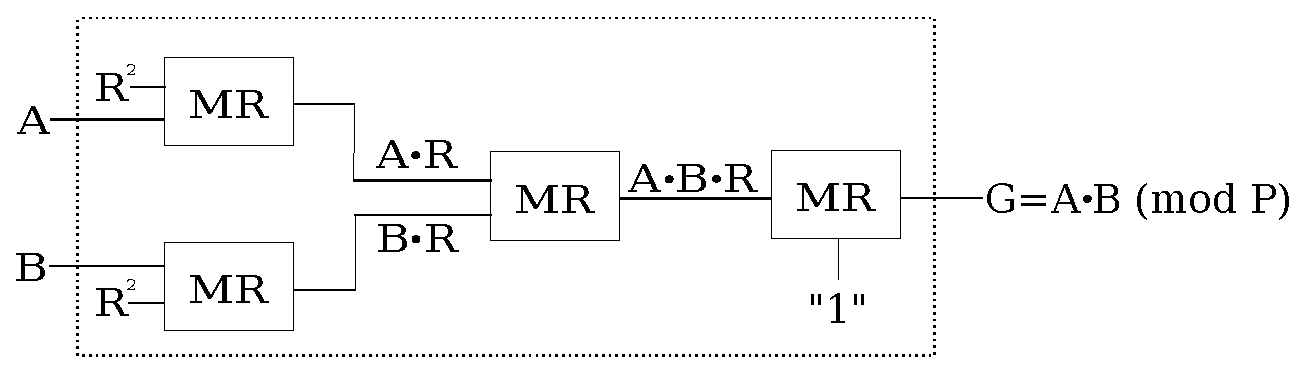
\includegraphics[scale=0.40]{figures/mmcircuit}
%	\end{center}
%	\caption{Montgomery multiplier over $\mathbb{F}_{2^k}$}
%	\label{fig:mm4}
%\end{figure}
Montgomery multipliers are typically designed hierarchically, as shown in Fig. \ref{fig:mm4}. 
If the hierarchy is known, it can be
exploited by computing the abstraction of each MR block in parallel, as shown in 
Table \ref{tbl:montBlkToolResults}.
In this table, 'BLK A' and 'B' denote the input MR blocks, 'BLK
Mid' denotes the middle block and 'BLK Out' is the output block. While
each block is an MR block, some have been simplified by
constant-propagation, hence they have
different sizes. First, a polynomial is extracted for each MR block
(gate-level to word-level abstraction), and then the approach is
re-applied at word-level to derive the input-output relation (solved
trivially in $< 1$ second). Our approach can extract the word-level
polynomial for up to 571-bit circuits! 

%\setlength{\abovecaptionskip}{3pt}
\begin{table}[hbt]
\begin{center}
{\small
\caption{Abstraction of flat Montgomery multipliers. Time given in seconds, memory given in MB. $TO$ = $3$ days ($259,200$ seconds.}
\label{tbl:montFlatToolResults}
%\noindent\resizebox{\textwidth}{!}{%
\begin{tabular}{|l|r|c|c|c|c|c|c|c|} 
\hline
\multicolumn{2}{|c|}{Size (k)}      &  163  &     233 &     283 &     409 & 571 \\
\multicolumn{2}{|c|}{\# of Gates}   & 184K  &    329K &    488K &    1.0M & 1.97M \\
%% \hline
%% \multirow{2}{*}{Singular} & Time    &    -     &    -    &    -    &    -    &    -      \\
%%                           & Max Mem &    -     &    -    &    -    &    -    &    -      \\
\hline
\multirow{2}{*}{Time} & Bug Free &   6,897  &  63,805 &  TO & TO  &   TO \\
                      & Buggy    &   6,961  &  64,009 &  TO & TO  &   TO      \\
\hline
\multicolumn{2}{|c|}{Max Memory} &     153  &     325 &     505 &    971  &   2,240   \\
\hline
\end{tabular}
%}
}
\end{center}
\vspace{-0.15in}
\end{table}

\begin{table}[hbt]
\begin{center}
{\small
\caption{Abstraction of Montgomery blocks. Time given in seconds, memory is given in MB. TO = 3 days (259,200 seconds)}
\label{tbl:montBlkToolResults}
%\noindent\resizebox{\textwidth}{!}{%
\begin{tabular}{|l|r|c|c|c|c|c|c|} 
\hline
\multicolumn{3}{|c|}{Circuit Size (k)}                          &    163 &      233 &     283 &     409 &     571 \\
\hline
\multicolumn{2}{|c|}{\multirow{4}{*}{\# of Gates}}    & Blk A   & 33K &   55K &  82K & 168K & 330K \\
\multicolumn{2}{|c|}{}                                & Blk B   & 33K &   55K &  82K & 168K & 330K \\
\multicolumn{2}{|c|}{}                                & Blk Mid & 85K &  163K & 241K & 502K & 980K \\
\multicolumn{2}{|c|}{}                                & Blk Out & 32K &   54K &  81K & 168K & 328K \\
\hline
%% \multirow{6}{*}{Singular}    & \multirow{4}{*}{Time}  & Blk A   & 22,860  &    -    &    -    &    -    &    -    \\
%%                              &                        & Blk B   & 19,476  &    -    &    -    &    -    &    -    \\
%%                              &                        & Blk Mid & 18,010  &    -    &    -    &    -    &    -    \\
%%                              &                        & Blk Out & 17,604  &    -    &    -    &    -    &    -    \\
%% \hhline{~-----------}
%%                              & \multicolumn{2}{|r|}{Total Time} & 77,950  &    -    &    -    &    -    &    -    \\
%%                              & \multicolumn{2}{|r|}{Max Mem}    & 58,266  &    -    &    -    &    -    &    -    \\
%% \hline
%                                                             163       233       283      409       571
\multirow{8}{*}{Time} &\multirow{4}{*}{Bug Free}& Blk A   &    25 &      142 &     330 &   1,322 &   5,371 \\
                      &                         & Blk B   &    25 &      141 &     329 &   1,335 &   5,241 \\
                      &                         & Blk Mid &    73 &      408 &     883 &   4,471 &  19,942 \\
                      &                         & Blk Out &    24 &      140 &     321 &   1,338 &   5,532 \\
\hhline{~-------}
                      &\multirow{4}{*}{Buggy}   & Blk A   &    26 &      142 &     331 &   1,323 &   5,372 \\
                      &                         & Blk B   &    26 &      141 &     330 &   1,336 &   5,421 \\
                      &                         & Blk Mid &   111 &      580 &   1,411 &   6,829 &  37,804 \\
                      &                         & Blk Out &    25 &      141 &     322 &   1,339 &   5,539 \\
\hline%{~-----------}
%\multicolumn{3}{|r|}{Total Time}                          &    636 &    1,909 &   8,186 &  34,002 &  87,458 \\
\multicolumn{3}{|r|}{Max Mem Per Blk}                      &    80 &      168 &    254 &     538 &   1,129 \\
\hline

\end{tabular}
%}
}
\end{center}
\vspace{-0.2in}
\end{table}

%A multiplier over $\Fkk$ can also be composed over the composite field
%$\Fm_{(2^m)^n}$, where $k = m\cdot n$. The input $A=a_0+a_1\alpha+\dots+a_{k-1}\alpha^{k-1}$ is 
%transformed into multiple word-level input blocks over $\Fm_{2^m}$, $A_0,A_1,\dots,A_{n-1}$,
%where each $A_i=a_{i0}+a_{i1}\beta+\dots+a_{i(m-1)}\beta^{m-1}$ 
%and $\beta$ is the primitive element of $\Fm_{2^m}$. The multiplier is then 
%composed of m-bit blocks, each of which is either an m-bit adder or an m-bit 
%multiplier over $\Fm_{2^m}$. 
%An example $4$-bit multiplier with designed over $\Fm_{(2^2)^2}$ is 
%seen in Figure \ref{fig:comp4ex}. 
To abstract a word-level representation of the 
composite field multiplier $\F_{(2^m)^n}$ [Fig. \ref{fig:comp4ex}], we
first apply our approach to abstract a word-level representation of each m-bit block. 
In the case of an adder, this abstraction is trivially computed in $1$ second. 
In the case of a multiplier, 
refer to our experimental results for Mastrovito multipliers for comparison (Table \ref{tbl:mastroToolresults})
as these are designed as $m$-bit Mastrovito blocks. Each abstraction can be computed independently. 
Once these word-level abstractions are known, the final abstraction over $\F_{(2^m)^n}$ is performed
using only word-level variables. 
%For this, a functional mapping from each 
%$A_i$ to $A$ is needed in the form $A_i=\F_i(A)$. This is computed in a similarly 
%to the bit-level functional mapping $a_i=\F_i(A)$ described in 
%Section \ref{sec:improve}, except here the property $A_i^{2^m}=A_i$ is exploited 
%instead of the property $a_i^2=a_i$.
The results of this final word-level abstraction of 
buggy and bug-free multipliers over composite fields are shown in 
Table \ref{tbl:compositeToolResults}.

%\centering
%\begin{subfigure}{.4\columnwidth}
%\includegraphics[width=\columnwidth]{example-image-a}%
%\caption{cap a}%
%\label{subfiga}%
%\end{subfigure}\hfill%
%\begin{subfigure}{.4\columnwidth}
%\includegraphics[width=\columnwidth]{example-image-b}%
%\caption{cap b}%
%\label{subfigb}%
%\end{subfigure}\hfill%
%\begin{subfigure}{.4\columnwidth}
%\includegraphics[width=\columnwidth]{example-image-c}%
%\caption{cap c}%
%\label{subfigc}%
%\end{subfigure}%
%\caption{The proper caption}
%\label{figabc}
%\end{figure*}



%\begin{figure*}[t]
%        \centering
%        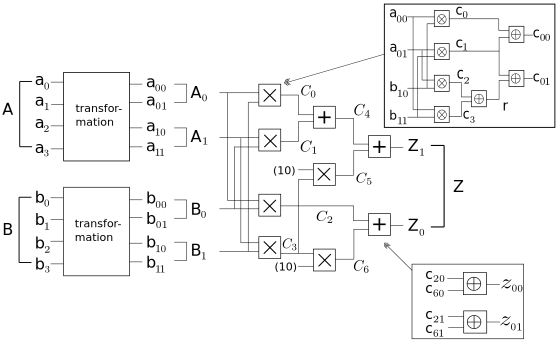
\includegraphics[width=.75\linewidth]{./figures/compMineSmall}
%        \caption{$4$-bit composite multiplier designed over $\Fm_{(2^2)^2}$}\label{fig:comp4ex}
%\end{figure*}

\begin{table}[!h]
\centering
{
\small
%\begin{tabular}{||c|c|c|c|c|c||c|c|c|c|c|c||c|c|c|c|c|c||} 
%\hline
%\multicolumn{6}{||c||}{64}&\multicolumn{6}{c||}{128}&\multicolumn{6}{c||}{256}\\
%\hline
%\multirow{2}{*}{$m$} &  \multirow{2}{*}{$n$} & \multicolumn{2}{c|}{Bug Free} & \multicolumn{2}{c||}{Buggy} &
%\multirow{2}{*}{$m$} &  \multirow{2}{*}{$n$} & \multicolumn{2}{c|}{Bug Free} & \multicolumn{2}{c||}{Buggy} &
%\multirow{2}{*}{$m$} &  \multirow{2}{*}{$n$} & \multicolumn{2}{c|}{Bug Free} & \multicolumn{2}{c||}{Buggy}   \\
%\hhline{~~----~~----~~----}
%     &       & Time    &   Mem   & Time     &   Mem &
%     &       & Time    &   Mem   & Time     &   Mem &
%     &       & Time    &   Mem   & Time     &   Mem\\
%\hline
%$2$  & $32$  & $4$     &  $4$    & $4$      & $10$  &
%$2$  & $64$  & $188$   & $11$    & $118$    & $32$  &
%$2$  & $128$ & $10,602$& $45$    & $10,617$ & $126$ \\
%\hline
%$4$  & $16$  & $7$     &   $5$   & $7$      & $11$  &
%$4$  & $32$  & $271$   &   $15$  &  $272$   & $36$  &
%$4$  & $64$  & $23,876$&   $61$  & $23,910$ & $142$ \\
%\hline
%$8$  & $8$  &  $9$     &  $5$    & $9$      & $11$  &
%$8$  & $16$ & $412$    &  $17$   &  $414$   & $38$ &
%$8$  & $32$ & $32,247$ &  $69$   & $32,293$ & $150$ \\
%\hline
%$16$ & $4$  & $11$     &  $5$    & $11$     & $11$  &
%$16$ & $8$  & $513$    & $19$    & $514$    & $40$ &
%$16$ & $16$ & $41,594$ & $74$    & $41,651$ & $155$ \\
%\hline
%$32$ & $2$  & $12$     &  $5$    & $12$     & $12$  &
%$32$ & $4$  & $545$    & $19$    & $546$    & $40$ &
%$32$ &  $8$ & $46,223$ & $75$    & $46,285$ & $156$ \\
%\hline
%   - &   -  &   -      &      -  &        - &      - &
%$64$ & $2$  & $563$    & $19$    &  $565$   & $40$&
%$64$ &  $4$ & $49,466$ & $75$    & $49,532$ &  $156$ \\
%\hline
%  -   &   - &   -      &    -    &    -     &     -  &
%  -   &   - &   -      &    -    &    -     &     -  &
%$128$ & $2$ & $55,440$ & $76$    & $55,513$ &  $157$ \\
%\hline
%\end{tabular}
%\begin{tabular}{|c|c|c|c|c|}
%\hline
%\multicolumn{5}{|c|}{64}\\
%\hline
%\multirow{2}{*}{$m$} &  \multirow{2}{*}{$n$} & \multicolumn{2}{c|}{Time} & Max \\
%\hhline{~~--~}
%     &       & Bug Free    &   Buggy   &   Mem \\
%\hline
%$2$  & $32$  & $4$     & $4$      & $10$  \\
%\hline
%$4$  & $16$  & $7$     & $7$      & $11$  \\
%\hline
%$8$  & $8$  &  $9$     & $9$      & $11$  \\
%\hline
%$16$ & $4$  & $11$     & $11$     & $11$  \\
%\hline
%$32$ & $2$  & $12$     & $12$     & $12$  \\
%\hline
%   - &   -  &   -      &        - &      -\\
%\hline
%  -   &   - &   -      &    -     &     - \\
%\hline
%\end{tabular}

\begin{tabular}{|c|c|c|c|c|}
\hline
\multicolumn{5}{|c|}{128}\\
\hline
\multirow{2}{*}{$m$} &  \multirow{2}{*}{$n$} & \multicolumn{2}{c|}{Time} & Max \\
\hhline{~~--~}
     &      & Bug Free & Buggy & Mem \\
\hline
 $2$ & $64$ &      $1$ &   $1$ & $4$ \\
\hline
 $4$ & $32$ &      $1$ &   $1$ & $2$ \\
\hline
 $8$ & $16$ &      $1$ &   $1$ & $2$ \\
\hline
$16$ &  $8$ &      $1$ &   $1$ & $2$ \\
\hline
$32$ &  $4$ &      $1$ &   $1$ & $2$ \\
\hline
$64$ &  $2$ &      $1$ &   $1$ & $3$ \\
\hline
  -  &   -  &   -      &   -   &  -  \\
\hline
  -  &   -  &   -      &   -   &  -  \\
\hline
  -  &   -  &   -      &   -   &  -  \\
\hline
\end{tabular}
\begin{tabular}{|c|c|c|c|c|}
\hline
\multicolumn{5}{|c|}{256}\\
\hline
\multirow{2}{*}{$m$} &  \multirow{2}{*}{$n$} & \multicolumn{2}{c|}{Time} & Max \\
\hhline{~~--~}
     &        & Bug Free & Buggy & Mem  \\
\hline
  $2$ & $128$ &     $15$ &  $15$ & $23$ \\
\hline
  $4$ &  $64$ &      $2$ &   $2$ &  $4$ \\
\hline
  $8$ &  $32$ &      $1$ &   $1$ &  $3$ \\
\hline
 $16$ &  $16$ &      $1$ &   $1$ &  $2$ \\
\hline
 $32$ &   $8$ &      $1$ &   $1$ &  $2$ \\
\hline
 $64$ &   $4$ &      $1$ &   $1$ &  $2$ \\
\hline
$128$ &   $2$ &      $1$ &   $1$ &  $2$ \\
\hline
  -   &   -   &       -  &    -  &   -  \\
\hline
  -   &   -   &       -  &    -  &   -  \\
\hline
\end{tabular}
\begin{tabular}{|c|c|c|c|c|}
\hline
\multicolumn{5}{|c|}{512}\\
\hline
\multirow{2}{*}{$m$} &  \multirow{2}{*}{$n$} & \multicolumn{2}{c|}{Time} & Max \\
\hhline{~~--~}
     &        & Bug Free & Buggy & Mem  \\
\hline
  $2$ & $256$ &    $406$ & $408$ & $90$ \\
\hline
  $4$ & $128$ &     $53$ &  $53$ & $25$ \\
\hline
  $8$ &  $64$ &      $8$ &   $8$ &  $4$ \\
\hline
 $16$ &  $32$ &      $2$ &   $2$ &  $4$ \\
\hline
 $32$ &  $16$ &      $1$ &   $1$ &  $3$ \\
\hline
 $64$ &   $8$ &      $1$ &   $1$ &  $3$ \\
\hline
$128$ &   $4$ &      $1$ &   $1$ &  $2$ \\
\hline
$256$ &   $2$ &      $1$ &   $1$ &  $2$ \\
\hline
  -   &   -   &      -   &   -   &   -  \\
\hline
\end{tabular}
\begin{tabular}{|c|c|c|c|c|}
\hline
\multicolumn{5}{|c|}{1024}\\
\hline
\multirow{2}{*}{$m$} &  \multirow{2}{*}{$n$} & \multicolumn{2}{c|}{Time} & Max \\
\hhline{~~--~}
      &       & Bug Free &  Buggy   &   Mem \\
\hline
  $2$ & $512$ & $11,883$ & $12,050$ & $414$ \\
\hline
  $4$ & $256$ &  $1,520$ &  $1,536$ & $106$ \\
\hline
  $8$ & $128$ &    $209$ &    $211$ &  $29$ \\
\hline
 $16$ &  $64$ &     $38$ &     $37$ &  $10$ \\
\hline
 $32$ &  $32$ &     $10$ &     $10$ &   $5$ \\
\hline
 $64$ &  $16$ &      $4$ &      $4$ &   $3$ \\
\hline
$128$ &   $8$ &      $2$ &      $2$ &   $3$ \\
\hline
$256$ &   $4$ &      $1$ &      $1$ &   $3$ \\
\hline
$512$ &   $2$ &      $1$ &      $1$ &   $3$ \\
\hline
\end{tabular}
}
\caption{Abstraction of bug-free Mastrovito multipliers over $\mathbb{F}_{(2^m)^n}$. Time is given in seconds. Memory is given in MB. $TO$ = more than $24$ hours = $86,400$ seconds. 
Note that abstractions of the $m$-bit blocks which compose the circuits are already known.}
\label{tbl:compositeToolResults}
\end{table}


\begin{table}[!hbt]
\begin{center}
{\small
\caption{Statistics of Designs over $\mathbb{F}_{(2^m)^n}$}
\label{tbl:stats}
\begin{tabular}{|c|c|c|c|c|c|c|c|} 
\hline
$n$ & 2 & 4 & 8 & 16 & 32 \\
\hline
\# of $\F_{2^m}$ Multipliers  & $6$ & $36$ & $168$ & $720$ & $2976$ \\
\hline
\# of $\F_{2^m}$ Adders       & $3$ & $27$ & $147$ & $675$ & $2883$  \\
\hline
\end{tabular}
}
\end{center}
\end{table}


%% For these
%% experiments, we used the Singular \cite{DGPS} computer algebra
%% tool. The results are shown in Table \ref{tab:ours}. The row
%% ``Compute-GB'' depicts the time required to compute the Gr\"obner
%% basis using the abstraction term order; whereas the row ``Improved-GB''
%% depicts the result of our improved, guided, approach using RATO. We
%% correctly identified $Z + A\cdot B$ as the only word-level polynomial
%% in the Gr\"obner basis $G'$, for up to 163-bit circuits over
%% ${\mathbb{F}}_{2^{163}}$. Similarly, the results for Montgomery
%% multipliers are shown in Table \ref{tab:mont}. Montgomery multipliers
%% are significantly larger than Mastrovito ones. The 163-bit circuit has
%% more than $91,000$ variables, which Singular cannot accommodate, as
%% its capacity is limited to $< 32767$ variables. Therefore, the largest
%% experiment was restricted to 128-bit Montgomery multipliers. 
%% These experiments were conducted  on a desktop with $2.40$GHz Intel
%% Core \texttrademark{$2$} Quad CPU with $8$GB memory running $64$-bit
%% Linux. 


The above experiments also demonstrate that we can perform equivalence
checking between Mastrovito (golden model) and Montgomery multiplier
(implementation) circuits, by deriving a canonical polynomial ($Z_1,
Z_2$)from each circuit independently and then checking if $Z_1 =
Z_2$, for up to 571-bit circuits. Our experiments have shown that contemporary 
approaches (BDDs, SAT, SMT, and AIG/ABC) show some success in bug-catching for these
kinds of circuits (particularly ABC). These experiments are shown in Table \ref{tab:satsmtbugcatch}.
Note that ABC uses random simulation for FRAIGing (functionally reducing AIGs), which
can catch a bug early if it is lucky.
However, full equivalence checking using any of these techniques failed even for 
16-bit circuits, as shown in Table \ref{tab:equivCheckFail}.

\begin{table}[!hbt]
\begin{center}
{\small
\caption{Bug-catching between a golden-model Mastrovito and buggy Montgomery circuit. 
Time given in seconds. TO = 3 days (259,200 seconds)}
\label{tab:satsmtbugcatch}
%\noindent\resizebox{\textwidth}{!}{%
\begin{tabular}{|l|c|c|c|c|c|c|} 
\hline
Circuit Size (k) &  64  &    163 &      233 &     283 &     409 &    571  \\
\hline
ABC              &  1     &    32  &     6    &   96    &     217 &    401  \\
\hline
Lingeling        &  1     &     8  &    362   & 12,728  &   3,323 & 23,298  \\
\hline
Picosat          & 15,235 &    TO  &    TO    &    TO   &     TO  &   TO    \\
\hline
Boolector        &  4     &    30  &    41    &   105   &    152  & 19,113  \\
\hline
CVC4             &  2     &    11  &    64    &  8,660  &    280  &    TO   \\
\hline
Z3               &  1     &    12  &    55    & 10,169  &    335  &    TO   \\
\hline
Yices            &  1     &     6  &     7    &   618   &    578  & 11,568  \\
\hline
\end{tabular}
%}
}
\end{center}
\vspace{-0.2in}
\end{table}

\begin{table}[!hbt]
\begin{center}
{\small
\caption{Equivalence checking between a golden-model Mastrovito and a bug-free Montgomery circuit. 
TO = 3 days (259,200 seconds)}
\label{tab:equivCheckFail}
%\noindent\resizebox{\textwidth}{!}
}
\end{center}
\vspace{-0.2in}
\end{table}

%between f, 
%as shown in Table III, these tools have shown
% In \cite{lv:date2012}, the authors
%have shown that this same equivalence checking experiment using
%contemporary approaches (BDDs, SAT, SMT, and AIG/ABC) is infeasible
%beyond 16-bit circuits (cf. Table I in \cite{lv:date2012}). 

%, the table is not reproduced here due to lack of space).   

%% \begin{table}[hbt!]
%% {\myfontsize
%% \begin{center}
%% \caption{\small Run-time for word-level abstraction from Mastrovito
%%   multipliers using our approach.  {\sc Singular} computer algebra
%%   tool is used for this experiments. Time is given in seconds. MO = out
%%   of memory.}  
%% \label{tab:ours}
%% \begin{tabular}{|l||c|c|c|c|c|c|c|} \hline 
%% Size $k$-bits& 16 & 32  & 64 & 128  &163\\
%% \hline
%% \#variables &$323$ &$1155$ &$4355$ &$16899$ &$27224$ \\
%% \hline
%% \#polynomials &$291$ &$1091$  &$4227$ &$16643$ &$26989$ \\
%% \hline
%% \#terms &$1793$ &$7169$  &$28673$ &$114689$ &$185984$ \\
%% \hline
%% Compute-GB & $124$ &$720$  &$MO$ &$MO$ &$MO$ \\
%% \hline
%% Improved-GB &$0.04$ &$1.6$ &$78$ &$4500$ &$18424$ \\
%% \hline
%% %Our approach: Bugs (s) & $0.04$ &$1.43$  &$114.86$ &$788.65$ &$3061$  &$9384$
%% % &$16368$\\
%% \hline
%% \end{tabular}
%% \end{center}
%% \vspace{-0.2in}
%% }
%% \end{table}



%% \begin{table}[htb!]
%% {\myfontsize
%% \begin{center}
%% \caption{ Runtime for word-level abstraction from Montgomery
%%   multipliers. TO = timeout of 10hrs. Time is given
%%   in seconds. $\ast$ denotes {\sc singular}'s capacity exceeded.} 
%% \label{tab:mont}
%% \begin{tabular}{|c||c|c|c|c|c|c|} \hline 
%% Operand size $k$ &  32 & 48 & 64 & 128 &163\\
%% \hline
%% \#variables     &$1194$     &$2280$     &$4395$     &$14122$  &$91246$\\
%% \hline
%% \#polynomials    &$1130$     &$2184$     &$4267$     &$13866$  &$89917$\\
%% \hline
%% \#terms          &$10741$    &$18199$    &$40021$    &$134887$ &$484738$\\
%% \hline \hline
%% %Compute-GB &$1.50$  &$11.03$    &$27.70$  &$10919$  &$\ast$\\
%% %\hline
%% Improved-GB    &$25$     &$1023$     &$3060$     &$11047$    &$\ast$\\
%% \hline
%% \end{tabular}
%% \end{center}
%% }
%% \end{table}

%\afterpage{\clearpage}
\FloatBarrier

\section{Limitations of the Abstraction Approach}

Our tools and approach performs very favorable for $\Fkk$ multiplier circuits and other 
functions designed over fields. These types of circuits are based on AND-XOR gate logic. 
Thus, the polynomials 
derived during the reduction procedures are very sparse. Since the  
complexity of the algorithm heavily depends on the density of the polynomials,
the worst-case is avoided in such designs.
In the case of bugs within these circuits, these polynomials increase in size, but are
still easily manageable. This is why the approach is applicable to
very large Galois field multipliers, both buggy and bug-free.

However, for random logic, especially logic containing chains of
OR gates, the polynomial becomes very dense. As a result, the algorithm begins 
to encounter the computational worst-case.  
This is best shown with a small example.

\begin{Example}
\begin{figure}[h]
        \centering
        \begin{subfloat}[][XOR logic]{%{0.25\textwidth}
                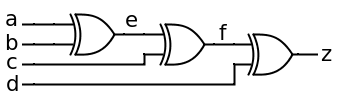
\includegraphics[width=0.25\textwidth]{./figures/xor-example}
                %\caption{XOR logic}
                \label{fig:xorEx}}
        \end{subfloat}%
        ~ %add desired spacing between images, e. g. ~, \quad, \qquad, \hfill etc.
          %(or a blank line to force the subfigure onto a new line)
        \begin{subfloat}[][OR logic]{%{0.25\textwidth}
                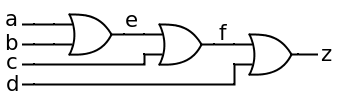
\includegraphics[width=0.25\textwidth]{./figures/or-example}
                %\caption{OR logc}
                \label{fig:orEx}}
        \end{subfloat}
        \caption{Logic comparisons}\label{fig:logicExmp}
\end{figure}


%\begin{figure}[!hbt]
%\centerline{
%\includegraphics[scale=0.5]{}
%}
%\caption{ XOR-based logic.}
%\label{fig:xorEx}
%\end{figure}
{\it 
Consider the circuit in Figure \ref{fig:xorEx}, which performs a 4-input
XOR function. Due to RATO, the monomial ordering of the variables is 
$z > f > e > d > c> b >a$. Thus, $z$ will be reduced in terms of the rest of the 
variables. The polynomials derived from the design are:
\begin{eqnarray}
f_1:z+f+d & f_2:f+e+c & f_3:e+b+a \nonumber
\end{eqnarray}
The reduction procedure $z \xrightarrow{f_1,f_2,f_3}_+ r$ will be computed as follows:
\begin{enumerate}
\item $z \xrightarrow{z+f+d} f+d$
\item $(f+d)\xrightarrow{f+e+c}e+d+c$
\item $(e+d+c)\xrightarrow{e+b+a}d+c+b+a$
\end{enumerate}
In each reduction, the output gate variable is removed and one copy of each 
input variable is added, leaving a sparse polynomial. Now consider the same 
circuit with the XOR gates replaced by OR gates, as shown in Figure \ref{fig:orEx}.

%\end{figure}
%\begin{figure}[!hbt]
%\centerline{
%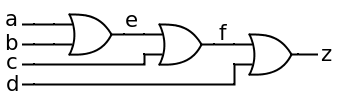
\includegraphics[scale=0.5]{./figures/or-example}
%}
%\caption{ OR-based logic.}
%\label{fig:orEx}
%\end{figure}
The monomial ordering stays the same, but the polynomials derived from each gate
have changed:

\begin{eqnarray}
f_1:z+fd+f+d & f_2:f+ec+e+c & f_3:e+ba+b+a \nonumber
\end{eqnarray}
The reduction procedure, $z \xrightarrow{f_1,f_2,f_3}_+ r$ is now computed as:
\begin{enumerate}
\item $z \xrightarrow{z+fd+f+d}fd+f+d$
\item $(fd+f+d)\xrightarrow{f+ec+e+c}f+edc+ed+dc+d$;\\
$(f+edc+ed+dc+d)\xrightarrow{f+ec+e+c}edc+ed+ec+e+dc+d+c$
\item $(edc+ed+ec+e+dc+d+c)\xrightarrow{e+ba+b+a}_+$\\ $dcba+dcb+dca+dba+dc+db+da+d+cba+cb+ca+c+ba+b+a$
\end{enumerate}
Each pass removes an output variable of the gate, but replaces it with two instances of each input variable.
This increases the density of the resulting polynomial exponentially.
}
\end{Example}

\section{Conclusions}

This chapter examined the data structures and algorithms implemented in a
custom software abstraction tool.
Abstraction of Galois field circuits using the custom tool has 
greatly better performance compared to using {\sc Singular} scripts. With it, we can
abstract circuits up to $1024$-bits, buggy or bug-free. Although a bug will 
generally substantially inflate the size of the resulting polynomial abstraction, 
the tool is not greatly hindered by the presence of bugs in a circuit.
However, for random logic, especially OR-based logic, the size of the polynomials tends 
to grow exponentially during the abstraction. Thus, the approach is infeasible for
circuits with OR-gate chains.
